% !TeX spellcheck = en_GB
% !TEX TS-program = xelatex
% !TEX encoding = UTF-8 Unicode
\documentclass[final,aspectratio=43]{beamer}

\usepackage[british]{babel}

\usetheme{metropolis}

\metroset{block=fill}

\usepackage{amsmath}
\usepackage{siunitx}
\usepackage{tabularx}


\usepackage{enumitem} 
%\setitemize{label=\usebeamerfont*{itemize item}%
%	\usebeamercolor[fg]{itemize item}
%	\usebeamertemplate{itemize item}}
\setlist[enumerate]{label=\arabic*.}

\usepackage{hyperref}
\usepackage{multicol}
\usepackage{graphicx}
\usepackage{textcomp}

\usepackage{listings}

\lstset{basicstyle=\ttfamily, % font style and size
  breakatwhitespace=false,
  breaklines=true,
  numbers=left,
  numberstyle=\small,
  numbersep=5pt,
  language=[LaTeX]TeX
}

\newcolumntype{L}[1]{>{\raggedright\let\newline\\\arraybackslash\hspace{0pt}}m{#1}}
\newcolumntype{C}[1]{>{\centering\let\newline\\\arraybackslash\hspace{0pt}}m{#1}}
\newcolumntype{R}[1]{>{\raggedleft\let\newline\\\arraybackslash\hspace{0pt}}m{#1}}



\title{An Introduction to \LaTeX}
%\subtitle{Non-linear Dynamic Behaviour of Plants for Sensing and Computing}
\date{28 September 2020}
\author{Olivier Pieters}
\institute{IDLab-AIRO -- Ghent University (UGent) -- imec\\
  Research Institute for Agriculture, Fisheries and Food (ILVO)}

%\usepackage{minted}
%\renewcommand\theFancyVerbLine{\tiny\arabic{FancyVerbLine}}

\begin{document}

\begin{frame}[plain]
\maketitle
\end{frame}

\begin{frame}{Contents}
    \begin{itemize}
    \item Why \LaTeX?
    \item Document structure and syntax
    \item Preamble
    \item A First Document in \LaTeX
    \item<2->Several breaks to keep everybody focussed :)
    \end{itemize}
\end{frame}

\begin{frame}{Why (not) \LaTeX?}
    \begin{columns}
    \begin{column}{0.5\linewidth}
        \begin{itemize}
            \item[+] High typographical quality
            \item[+] Separate \emph{content} from \emph{layout} (WYSIWYM vs.\ WYSIWYG)
            \item[+] Modularity
            \item[+] Open-source, secure, accessible freely
            \item[+] Mathematics
            \item[-] Learning curve
            \item[-] Rapid document creation
        \end{itemize}
    \end{column}%
        \begin{column}{0.5\linewidth}
            \centering
            \includegraphics[width=\linewidth]{figures/latex-vs-word}
        \end{column}
    \end{columns}
\end{frame}

\begin{frame}{More Profession Output}
    \begin{columns}
        \begin{column}{0.5\linewidth}
            \begin{center}
            \onslide<2->{\Huge\LaTeX}
            
            
\includegraphics[width=0.4\linewidth]{figures/kerning_latex}
            
            
\includegraphics[width=\linewidth]{figures/sc_latex}
            
            
\includegraphics[width=\linewidth]{figures/ligatures_latex}
            
            \end{center}
        \end{column}%
        \begin{column}{0.5\linewidth}
            \begin{center}
            \onslide<2->{\Huge Word}
            
            
\includegraphics[width=0.4\linewidth]{figures/kerning_word}
            
            
\includegraphics[width=\linewidth]{figures/sc_word}
            
            
\includegraphics[width=\linewidth]{figures/ligatures_word}
            
            \end{center}
        \end{column}
    \end{columns}
\end{frame}

\begin{frame}{More Profession Output}
    \centering
    \renewcommand{\arraystretch}{2}
    \begin{tabularx}{0.9\linewidth}{X@{\hskip 1cm}X}
    {\Huge\LaTeX} & {\Huge Word} \\
    No double spaces & Double Spaces \\
    Consistent paragraph spacing & User most use consistent number of line breaks \\
    More natural spacing after a full stop & Same spacing after full stop \\
    \end{tabularx}
\end{frame}

\begin{frame}{Modularity}
    \begin{block}{\LaTeX\ vs.\ Word -- structure}
        Multiple documents (images, sections, tabular data)
    \end{block}
    
    \onslide<2->{
    \begin{block}{\LaTeX\ vs.\ Word -- editing}
        Source code is edited directly \textrightarrow\ no speed loss in large documents (though compilation time increases)
    \end{block}
    }
    
    \onslide<3->{
    \begin{block}{\LaTeX\ vs.\ Word -- tools}
        Multiple tools work together (e.g.\ bibliography, index, abbreviations)
    \end{block}
    }
\end{frame}

\begin{frame}{Check your Journal!}
    \begin{alertblock}{Journal}
        Always make sure your journal accepts PDF and/or \LaTeX\ submissions \emph{before} starting on a document.
    \end{alertblock}
    
    \onslide<2->{
    \begin{alertblock}{Formatting}
        Try to use the formatting of the journal by reading the guidelines online. This saves a late conversion (and all associated issues).
    \end{alertblock}
    }
\end{frame}

\begin{frame}[fragile]{A Simple Document}
    \vspace*{10pt}
    \begin{columns}
    \hfill
    \begin{column}{0.45\linewidth} 
        \lstinputlisting[numbers=left,numberstyle=\tiny,basicstyle=\tiny\ttfamily]{code/basic-document.tex}
    \end{column}%
    \begin{column}{0.5\linewidth}
        \fbox{\includegraphics[width=0.95\linewidth]{code/basic-document}}
    \end{column}
    \end{columns}
\end{frame}

\begin{frame}[fragile]{Some Syntax}

    \onslide<1->{
        \begin{block}{Macro}
           Starts with a backslash and can have some arguments \texttt{\textbackslash macro[optional]\{required\}}
        \end{block}
    }
    
    \onslide<2->{
        \begin{block}{Environment}
          Starts with \texttt{\textbackslash begin\{environment\}[optional keys]}
          
          Stops at \texttt{\textbackslash end\{environment\}}
        \end{block}
    }
    
    \onslide<3->{
        \begin{alertblock}{Special characters (subset)}
            \texttt{\textbackslash \@ \# \_ \&  \% \{ \}}
        \end{alertblock}
    }
    \onslide<4->{
        \begin{alertblock}{Strings}
            No special treatment of strings like in most programming languages, everything is \emph{some} kind of string
        \end{alertblock}
    }
\end{frame}

\begin{frame}{\LaTeX\ is not a programming language}
\begin{alertblock}{Important!}
    While \LaTeX\ might resemble a programming language, it is not a programming language but a \emph{typesetting system} built on top the programming language \TeX.
\end{alertblock}
\end{frame}

\begin{frame}[fragile]{Document Structure}
    \begin{block}{Preamble}
     set certain options and settings and include packages that are needed in the rest of the document, everything \emph{before} \texttt{\textbackslash begin\{document\}}
    \end{block}
    
    \begin{block}{Contents}
        the contents of the document, everything \emph{after} \texttt{\textbackslash begin\{document\}} and \emph{before} \texttt{\textbackslash end\{document\}}
    \end{block}
\end{frame}

\begin{frame}[fragile]{The Preamble}
    \lstinputlisting[firstline=1,lastline=10]{code/basic-document.tex}
\end{frame}

\begin{frame}[fragile]{The Preamble - explained}
   \onslide<1->{\lstinputlisting[firstline=1,lastline=1]{code/basic-document.tex}}
   \only<2>{Define the document type, default font size and language. Common document types are:
   
   \begin{itemize}
   \item \texttt{article}
   \item \texttt{book} (and \texttt{report})
   \item \texttt{letter}
   \item \texttt{beamer}
   \item many journals have their own class (e.g.\ \texttt{mdpi}, \texttt{elsarticle})
   \end{itemize}
   
   The following font sizes are supported by default: \texttt{10pt} (default), \texttt{11pt} and \texttt{12pt}
   
   Other options include settings for the number of columns, two sided typesetting\ldots}
   \onslide<3->{\lstinputlisting[firstline=3,lastline=5,firstnumber=last]{code/basic-document.tex}}
   \only<4>{%
       Load packages (\texttt{\textbackslash usepackage})
       \begin{itemize}
           \item \lstinline|geometry|: page layout (A4)
           \item \lstinline|babel|: language settings (hyphenation etc.)
           \item \lstinline|lipsum|: dummy text (normally not loaded)
       \end{itemize}%
   }
   \onslide<5->{\lstinputlisting[firstline=7,lastline=8,firstnumber=last]{code/basic-document.tex}}
   \only<6>{Define the title of this document and the author}
   \onslide<7->{\lstinputlisting[firstline=10,lastline=10,firstnumber=last]{code/basic-document.tex}}   
   \only<8>{Start the actual document}
   \onslide<9->{\lstinputlisting[firstline=12,lastline=12,firstnumber=last]{code/basic-document.tex}} 
   \onslide<10->{\lstinputlisting[firstline=26,lastline=26,firstnumber=last]{code/basic-document.tex}} 
\end{frame}

\begin{frame}{Overleaf}
    \centering
    
\includegraphics[width=0.7\linewidth]{figures/overleaf}
    \url{https://www.overleaf.com}
    
    Local installation is also possible: 
    \url{https://www.latex-project.org/get/}
\end{frame}

\begin{frame}{Writing a First Document}
    \centering
    \emph{\Large Exercise}
    
    \onslide<2->{Journal article in \textit{Computer and Electronics in Agriculture}}
    
    \onslide<3->{\includegraphics[width=3cm,page=1]{elsdoc} \includegraphics[width=3cm,page=2]{elsdoc} \includegraphics[width=3cm,page=3]{elsdoc}
    
    \url{https://ctan.org/pkg/elsarticle}}
\end{frame}

\begin{frame}[fragile]{The preamble (for now)}
    \lstinputlisting[firstline=6,lastline=9]{example/article.tex}
    
    \lstinputlisting[firstline=58,lastline=58,firstnumber=last]{example/article.tex}
\end{frame}

\begin{frame}[fragile]{Staring the Document}
    \lstinputlisting[firstline=62,lastline=66]{example/article.tex}
\end{frame}

\begin{frame}[fragile]{Authorship}
    \lstinputlisting[firstline=68,lastline=75,firstnumber=last]{example/article.tex}
\end{frame}

\begin{frame}[fragile]{Addresses}
    \lstinputlisting[firstline=77,lastline=78,firstnumber=last]{example/article.tex}
\end{frame}

\begin{frame}[fragile]{Abstract (part 1)}
    \lstinputlisting[firstline=80,lastline=80,firstnumber=last]{example/article.tex}
    
    Abstract contents added later.
    
    \lstinputlisting[firstline=106,lastline=106,firstnumber=last]{example/article.tex}
\end{frame}

\begin{frame}[fragile]{Highlights}
    \lstinputlisting[firstline=108,lastline=111,firstnumber=last]{example/article.tex}
\end{frame}

\begin{frame}[fragile]{Keywords}
    \lstinputlisting[firstline=113,lastline=115,firstnumber=last]{example/article.tex}
\end{frame}

\begin{frame}[fragile]{Ending the Document (for now)}
\lstinputlisting[firstline=117,lastline=117,firstnumber=last]{example/article.tex}
\lstinputlisting[firstline=407,lastline=407,firstnumber=last]{example/article.tex}

\textrightarrow\ Compile the document and see the output!
\end{frame}

\begin{frame}[fragile]{Adding the abstract}
Inside the \lstinline|abstract| environment, add:
\begin{lstlisting}[basicstyle=\tiny,numbers=none]{latex}
In perennial ryegrass breeding programs, dry matter yield (DMY) of
individual plots is monitored destructively at the different cuts or
derived from non-destructive canopy height measurements using devices
like rising plate meters (RPM). These approaches both have constraints.
Destructive sampling implies low temporal resolution, restraining the
study of dry matter accumulation rates, while RPM measurements are
influenced by the canopy structure and limit intra-field variability
identification. We present a phenotyping methodology, based on the use
of an affordable RGB camera mounted on an Unmanned Aerial Vehicle (UAV),
to monitor the spatial and temporal evolution of canopy height and to
estimate DMY. Weekly flights were carried out from April to October
above a field comprising a diverse set of accessions. To test the
capability of the model extracted from the data to estimate canopy height, 
8 ground control points and 28 artificial height references were placed 
at different locations. Accurate flights with an RMSE as low as 0.94 cm were
achieved. In addition, canopy height was recorded using an RPM and
destructive biomass samples were collected. Different models (linear,
multiple linear, principal components, partial least squares regression
and random forest) were used to predict DMY and their performance was
evaluated. The best estimations were obtained by combining variables
including canopy height, vegetation indices and environmental data in a
multiple linear regression (${R^2 = 0.81}$). All models built using UAV data
obtained a lower RMSE than the one using RPM data. The approach
presented is a possibility for breeders to incorporate new information
in their selection process.
\end{lstlisting}

\end{frame}

\begin{frame}[fragile]{Math in \LaTeX}
\onslide<1->{
\begin{block}{Inline math}
    Use \texttt{\$ ... \$} or \texttt{\textbackslash( ... \textbackslash)} for inline math
\end{block}

\begin{block}{Formulas}
    Use the \texttt{equation} environment or \texttt{\textbackslash[ ... \textbackslash]} for formulas etc. 
\end{block}
}

\only<2>{
\begin{alertblock}{Legacy code}
    Sometimes, you might see \texttt{\$\$ math \$\$}, which is old and \emph{deprecated} code that should be avoided, but gives the same result (mostly).
\end{alertblock}
}

\onslide<3->{It's always a good idea to load the \texttt{amsmath} package.}

\onslide<4->{
($R^2 = 0.81$) requires additional attention:


\begin{columns}
    \begin{column}{0.5\linewidth}
        \centering
        \lstinline|$R^2 = 0.81$|
    \end{column}%
    \begin{column}{0.5\linewidth}
        \centering
        $R^2 = 0.81$
    \end{column}
\end{columns}
}

\onslide<5->{
But now the R is in italics...

\begin{columns}
    \begin{column}{0.5\linewidth}
        \centering
        \texttt{\$\textbackslash text\{R\}\^{}2 = 0.81\$}
    \end{column}%
    \begin{column}{0.5\linewidth}
        \centering
        $\text{R}^2 = 0.81$
    \end{column}
\end{columns}
}

\onslide<6->{
There might still be a line break somewhere...

\begin{columns}
    \begin{column}{0.5\linewidth}
        \centering
        \texttt{\$\{\textbackslash text\{R\}\^{}2 = 0.81\}\$}
    \end{column}%
    \begin{column}{0.5\linewidth}
        \centering
        ${\text{R}^2 = 0.81}$
    \end{column}
\end{columns}
}
\end{frame}

\begin{frame}[fragile]{Some formatting issues}
    \centering
    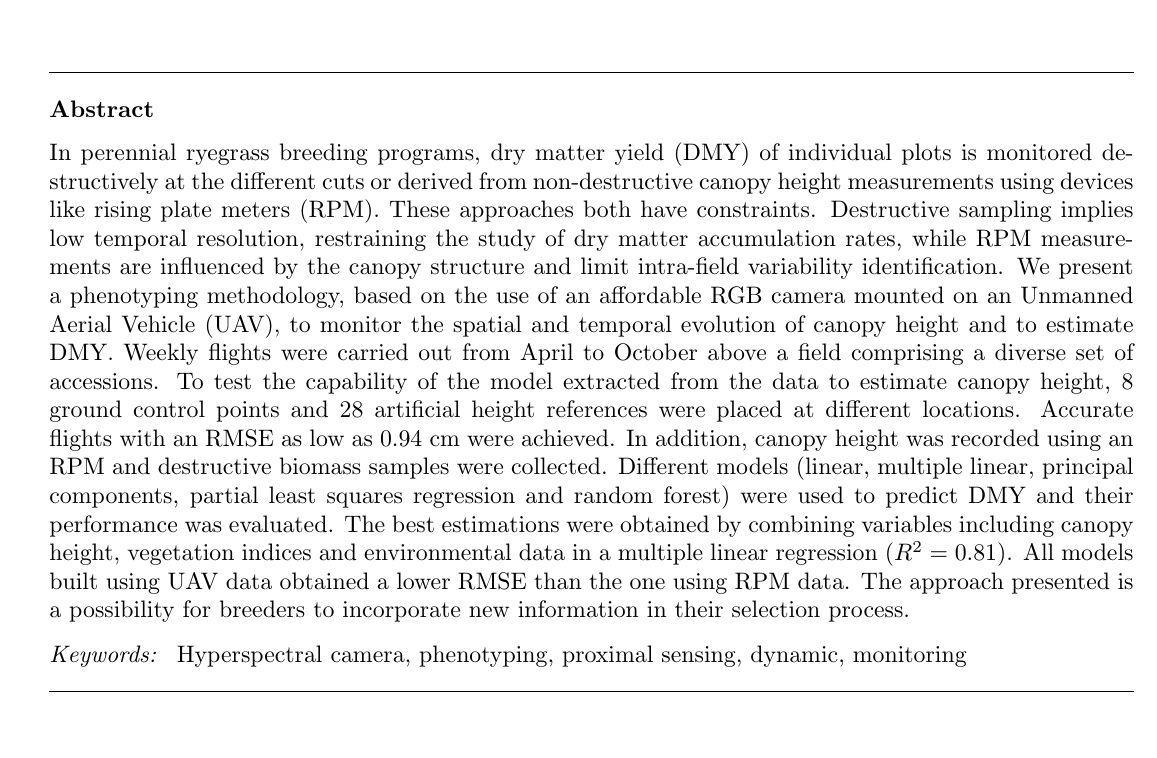
\includegraphics[width=\linewidth]{figures/abstract-issues}
\end{frame}


\begin{frame}{The Abstract -- Potential Issues}

\begin{columns}
    \begin{column}{0.5\linewidth}
    \onslide<1->{
        \begin{itemize}
            \item \lstinline|8 ground|
            \item \lstinline|28 artificial|
            \item \lstinline|0.94 cm|
        \end{itemize}
    }
    \end{column}\onslide<3->{%
    \begin{column}{0.5\linewidth}
        \begin{itemize}
            \item \lstinline|8~ground|
            \item \lstinline|28~artificial|
            \item \lstinline|0.94~cm|
        \end{itemize}
    \end{column}
    }
\end{columns}
\vspace{0.5cm}
\onslide<2->{
    \begin{block}{Non breaking space}
        Add a tilde (\texttt{\~{}}) when you need a space, but do not want the line to break
    \end{block}
}
    
\end{frame}

\begin{frame}[fragile]{Sections}
    \lstinline|\section{Materials and Methods}|
    \lstinline|\subsection{Data Sources}|
    \lstinline|\subsubsection{Handheld Camera}|
    \onslide<2->{
    \begin{block}{Non-numbered sections}
        Starred version: \texttt{\textbackslash section*\{Materials and Methods\}}
    \end{block}
    }
    \onslide<3->{
    \begin{block}{Labelling}
        Create a label to refer to this section in the text: \texttt{\textbackslash label\{materials-and-methods\}}
    \end{block}
    }
    \onslide<4->{
    \begin{alertblock}{Beware of special characters}
        Never use \%, \_ or spaces to label items. Use a dash or CamelCase to distinguish words. Sometimes it's useful to add a class: \texttt{\textbackslash label\{sec:materials-and-methods\}}.
    \end{alertblock}
    }
\end{frame}

\begin{frame}[fragile]{The introduction}

Add the contents to the introduction and hit compile.

\onslide<2->{\begin{block}{New Macros}
\begin{columns}
    \begin{column}{0.5\linewidth}
        \begin{itemize}[label={}]
            \item \texttt{\textbackslash citep}
            \item \texttt{\textbackslash citet}
            \item \texttt{\textbackslash textit}
            \item \texttt{\textbackslash textbf}
            \item \texttt{\textbackslash textsubscript}
            \item \texttt{\textbackslash emph}
        \end{itemize}
    \end{column}
    \begin{column}{0.5\linewidth}
        \begin{itemize}[label={}]
            \item normal citation
            \item inline citation
            \item italics
            \item bold
            \item subscript
            \item put the emphasis on this (usually in italics)
        \end{itemize}
    \end{column}
\end{columns}
\end{block}
}

\end{frame}

\begin{frame}{Citations: Workflow}
\begin{block}{Biber / biblatex}
    External programme that processes the citations in this document, based on \texttt{.bib}-file.
\end{block}

\onslide<2->{
Workflow:

\begin{enumerate}
    \item Create a database in Mendeley/Zotero with all your articles
    \item Export database to \texttt{.bib}-file
    \item Reference \texttt{.bib}-file in LaTeX
    \item Add references to citations using e.g.\ \texttt{\textbackslash cite}, \texttt{\textbackslash citep}
    \item Compile \LaTeX\ document at least once
    \item Run biber/biblatex
    \item Compile \LaTeX\ document at least once
\end{enumerate}
}

\onslide<3->{
But.. Overleaf manages this for you!
}

\end{frame}


\begin{frame}[fragile]{Adding Citations}
    \begin{block}{Default management}
        \texttt{\textbackslash cite\{key\}} \texttt{\textbackslash citet\{key\}} \texttt{\textbackslash citep\{key\}}
    \end{block}
    
    \begin{block}{Set the bibliography style}
        \texttt{\textbackslash bibliographystyle\{elsarticle-harv\}} many styles are predefined
    \end{block}
    
    \begin{block}{Load the \texttt{.bib}-file}
        \texttt{\textbackslash bibliography\{bibliography\}} notice that the file extension is emitted!
    \end{block}
    
%    \begin{block}{(Sometimes) typeset the bibliography}
%        \texttt{\textbackslash printbibliography}
%    \end{block}

    \begin{block}{Misc}
        This is the \texttt{natbib} workflow, \texttt{bibtex} and \texttt{biblatex} have a similar workflow.
    \end{block}
\end{frame}

\begin{frame}{Adding Materials and Methods}
    Let's increase the interactivity a bit.
    
    Open the Word document next to the LaTeX document and we'll covert it ourselves.  
\end{frame}


\begin{frame}[fragile]{Adding Figures}
    \begin{block}{\LaTeX\ uses floats}
        There is no direct relationship between figure location and placement in \LaTeX, figures float around in the document and are optimally placed based on references and surrounding text. 
    \end{block}
    
    \begin{lstlisting}[basicstyle=\ttfamily\small]
\begin{figure}[ht]
    \centering
    \includegraphics[width=7.5cm]{media/image6.png}
    \caption{Pearson correlation map...}
    \label{fig:pearson-correlation-map}
\end{figure}
    \end{lstlisting}
    
    \begin{block}{Referencing in the text}
        \texttt{Fig.\~{}\textbackslash ref\{fig:pearson-correlation-map\}}
    \end{block}
\end{frame}

\begin{frame}{Lengths in \LaTeX}
    \centering
    \begin{tabular}{ccc}
        long name & \LaTeX\ unit & description \\
        \hline
        centimetres & cm & the SI unit\\
        millimetres & mm & the SI unit\\
        inches & in & the empirical unit\\
        point & pt & based on the font size\\
        with of an \emph{m} & em & advanced use \\
        height of an \emph{x} & ex & advanced use\\
    \end{tabular}
    
    \onslide<2->{But one can also use predefined lengths
    
    \begin{tabular}{cc}
        macro & description \\
        \hline
        \texttt{\textbackslash linewidth} & length of one line of text\\
        \texttt{\textbackslash textheight} & height of the text on a page\\
        \texttt{\textbackslash paperwidth} & width of the page \\
        \texttt{\textbackslash paperheight} & height of the page\\
    \end{tabular}
    
    }
\end{frame}

\begin{frame}{Float placement in \LaTeX}
    \centering
    \begin{tabular}{cc}
        specifier & description \\
        \hline
        t & top\\
        b & bottom\\
        p & separate page\\
        h & here\\
        ! & really here \\

    \end{tabular}
\end{frame}

\begin{frame}{Nicely formatted units in \LaTeX}
    \begin{block}{New package}
        \texttt{siunitx} is a page that can be used to format numbers and units.
    \end{block}

    \SI{1.00 x 0.70 x 1.10}{\metre}\\
    \texttt{\textbackslash SI\{1.00 x 0.70 x 1.10\}\{\textbackslash metre\}}\\
    \texttt{\$1.00 \textbackslash text\{m\} \textbackslash times 0.70 \textbackslash text\{m\} \textbackslash times 1.10 \text\{m\}\$}
    
    \SIlist{11;33}{\celsius}\\
    \texttt{\textbackslash SIlist\{11;33\}\{\textbackslash celsius\}}\\
    \texttt{\$11\^{}\{\textbackslash circ\}\textbackslash text\{C\}\$ and \$33\^{}\{\textbackslash circ\}\textbackslash text\{C\}\$}
\end{frame}

\begin{frame}[fragile]{Adding Tables}
    \begin{lstlisting}[basicstyle=\ttfamily\small]
\begin{table}[!ht]
    \centering
    \caption{Best MLR to predict DMY...}
    \label{tab:MLR}
    \begin{tabular}{lcr}
        a & b & c \\
    \end{tabular}
\end{table}
    \end{lstlisting}
    
    \begin{block}{Column separator}
        \texttt{\&} is used to go to the next column
    \end{block}
    
    \begin{block}{Row separator}
        \texttt{\textbackslash\textbackslash} is used to go to the next row
    \end{block}
\end{frame}

\begin{frame}[fragile]{Table Options}
    \begin{tabular}{cL{10cm}}
    specifier & description \\
    \hline
    l & align content to the left \\
    c & centre content \\
    r & align content to the right \\
    | & vertical separator (do not use this!) \\
    @\{\} & specify column separation (usually not needed, e.g.\ \texttt{\textbackslash hskip 1cm})\\
    \end{tabular}

    \begin{alertblock}{Newlines}
        \texttt{\textbackslash\textbackslash} is also used to force a line break. Use \texttt{\textbackslash newline} instead in tables. The default table environment does \emph{not} support automated line breaks. There are more capable ones though.
    \end{alertblock}
\end{frame}


\begin{frame}{Defining New Commands}

Typing the same long sequence over and over again can get tiring. \LaTeX\ is expendable, so let's define a new command.

\texttt{\textbackslash usepackage\{xparse\}}
\texttt{\textbackslash NewDocumentCommand\{\textbackslash Tair\}\{\}\{T\textbackslash textsubscript\{air\}\}}
\texttt{\textbackslash NewDocumentCommand\{\textbackslash english\}\{m\}\{T\textbackslash textit\{\#1\}\}}

\end{frame}

\begin{frame}{So much more...}
    While you now know the basics, there's a lot more to be said and done

    \begin{itemize}
        \item<+-> Create figures in \LaTeX
        \item<+-> Use CSV data to make plots and tables
        \item<+-> Multi-file documents
        \item<+-> Advances references and options
        \item<+-> Lua scripting
        \item<+-> Advanced mathematical typesetting
        \item<+-> Slide shows
        \item<+-> Special packages for chemistry, linguistics, genetics
    \end{itemize}
\end{frame}

\begin{frame}{Questions and suggestions}

Are there things that we did not cover but that you think are essential?

\end{frame}


%
%\begin{frame}[fragile]{Filling Tables}
%\begin{lstlisting}[basicstyle=\ttfamily\small]
%\begin{tabular}{ccccc}
%\toprule
%variable set & variable   & mean ± SD          \\
%             &            &                    \\
%\midrule
%             & DM         & 3233.38 ± 1613.8   \\
%\midrule
%($\beta_0$)  &            &                    \\
%\midrule
%CHMv         & CH\_P50    & 205.42 ± 89.9      \\
%             & CH\_stdev  & 20.15 ± 10.9       \\
%\midrule
%VIv          & ExG\_stdev & 0.08 ± 0.02        \\
%\bottomrule
%\end{tabular}
%    \end{lstlisting}
%\end{frame}
%
%
\end{document}
